
%----------------------------------------------------------------------
% SECTION Firmware ESP32
%----------------------------------------------------------------------

\section{Firmware ESP32}
%\textcolor{red}{Wie wurde die Firmware auf dem ESP32 umgesetzt? Kurze Einleitung noch schreiben}

Die Firmware für den ESP32-S3 wurde mithilfe der ESP-IDF, dem IoT Development Framework, geschrieben. Dabei wurde die Integration von FreeRTOS sowie das Aufsetzen eines Bluetooth GATT-Servers programmiert. 

In Abbildung \ref{fig:FSMEinleitung} ist der Aufbau der Firmware grob schematisch zu sehen. Der Einstiegspunkt bietet dabei die \textit{app\_main()} Funktion, welche die Peripherien initialisiert und drei Tasks erstellt. Die main()-Funktion ist damit abgeschlossen und der Scheduler übernimmt die restliche Ausführung des Programms. Das Symbol in der rechten unteren Ecke in T2 zeigt an, dass dieser Task eine Statemachine umfasst. Auf die verschiedenen Tasks wird in diesem Abschnitt eingegangen.

\begin{figure}[H]
    \centering
    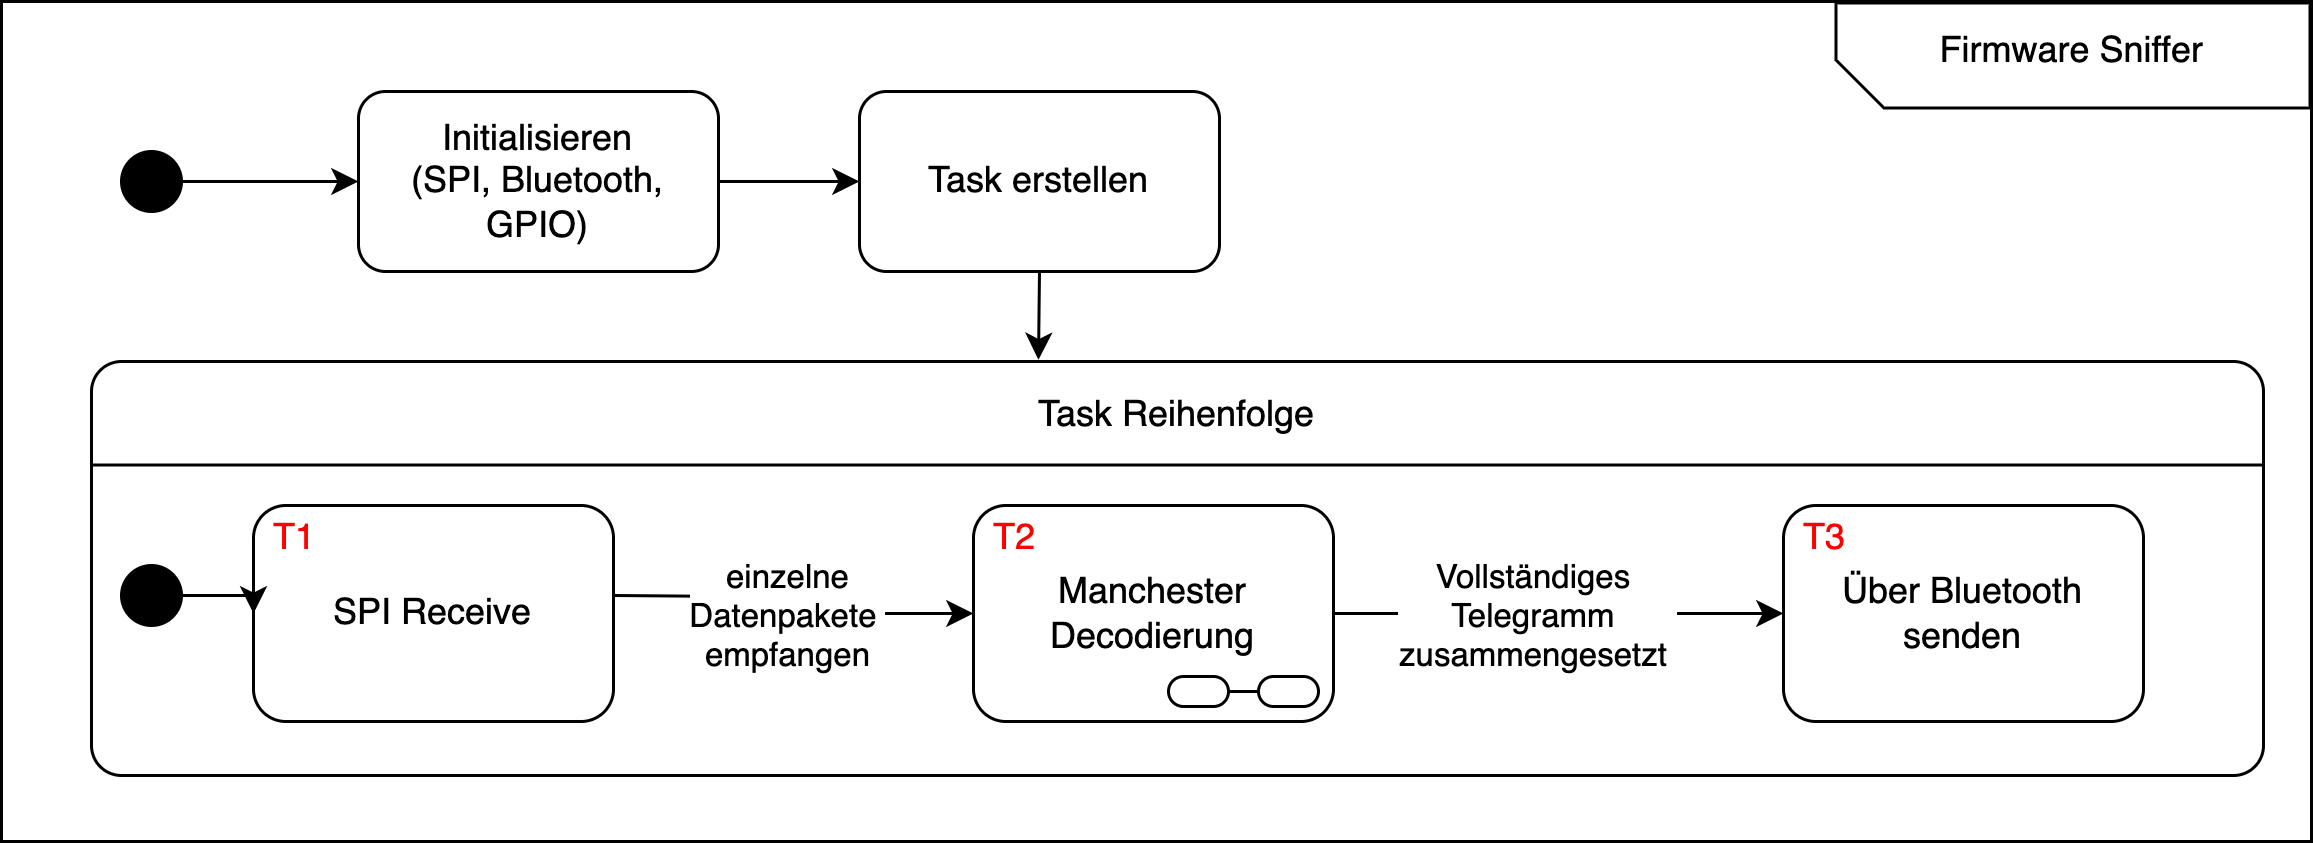
\includegraphics[width=0.9\linewidth]{Figures/Chap3/ESP/Einleitung/FSM_Einleitung.png}
    \caption{Ablaufdiagramm Firmware Sniffer von Programmeinstieg bis Task}
    \label{fig:FSMEinleitung}
\end{figure}

\subsection{Real Time Operating System (FreeRTOS) auf ESP32}
%\textcolor{red}{Wie wurde das FreeRTOS benutzt, um die Zeitkritische Aufgaben zu lösen? Welche Tasks und welche FSM arbeiten in den jeweiligen Cores?}


Für dieses Projekt kam FreeRTOS zum Einsatz, das bereits in der ESP-IDF, der Entwicklungsumgebung für den ESP32-S3, integriert ist. \cite{FREERTOS_IDF_API} In diesem Abschnitt werden die Umsetzung des Betriebssystems und die genutzten FreeRTOS-Elemente beschrieben, um den Betrieb zu ermöglichen.

\subsubsection{Task}
Es werden Tasks definiert, welche von einem Scheduler anschliessend gemanagt und aufgerufen werden. Für die Ausführung der Hauptaufgaben auf dem Sniffer wurden 3 Tasks gemäss Tabelle \ref{tab:TaskDefinitonen} definiert.

\begin{table}[H]
    \centering
    \begin{tabular}{|c||c|c|c|}
        \hline
        Funktionspointer & spi\_receive  & mvb\_manch\_decode & bt\_send\\ 
        \hline
        Name Task  & "'spi\_receive"' & "'mvb\_manch\_decode"' & "'bt\_send"'\\ 
        \hline
        Stackgrösse & 10000 & 10000 & 10000\\ 
        \hline
        Parameter & NULL & NULL & NULL\\ 
        \hline
        Priorität & 3 & 2 & 1\\ 
        \hline
        Handle & NULL & NULL & NULL\\ 
        \hline
    \end{tabular}
    \caption{Task Definitionen FreeRTOS}
    \label{tab:TaskDefinitonen}
\end{table}

Der Task \textit{spi\_receive} und \textit{mvb\_manch\_decode} erhalten beide eine grössere Priorität als der Task \textit{bt\_send}. Wie in Abbildung \ref{fig:ReineDaten} zu sehen ist, gibt es Zeitabschnitte, in denen viele Daten verarbeitet werden müssen, gefolgt von einer Idle-Periode. In der Idle-Zeit hat der Task \textit{bt\_send} die Möglichkeit, Telegramme über Bluetooth herauszuschicken und soll nicht in einer Periode, wo viele Daten kommen, die CPU beanspruchen.


\subsubsection{Queue}
\label{subsub:Queue}
Für den primären Datenaustausch zwischen den Tasks werden Queues verwendet. Wenn ein Task von einer leeren Queue lesen will, wird dieser in den \textit{blocking-state} versetzt. Dadurch gibt dieser Task die CPU frei und wird erst wieder aufgerufen, wenn sich ein Element in der Queue befindet.\cite{FREERTOS_QUEUE}

Für die Intertask-Kommunikation wurden zwei Queue definiert. In Abbildung \ref{fig:QueueSchema} ist eine schematische Darstellung des Datenflusses gezeigt.


\begin{figure}[H]
    \centering
    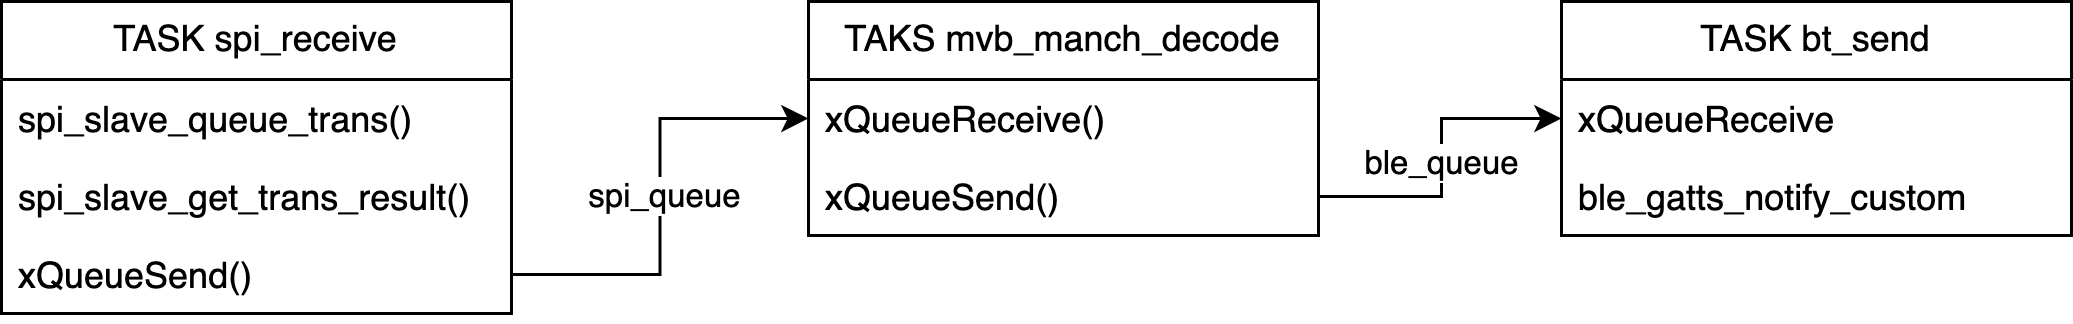
\includegraphics[width=0.9\linewidth]{Figures/Chap3/ESP/FreeRTOS/Queue.png}
    \caption{Schematische Darstellung der verwendeten Queues}
    \label{fig:QueueSchema}
\end{figure}

Die \textit{spi\_queue} fasst 64 Werte à 16 Bit. Die Wahl von 16 Bit basiert auf der Verarbeitung durch den Task \textit{mvb\_manch\_decode}. Die Grösse von 64 wurde gewählt, damit ein möglichst grosser Buffer ansteht und keine Daten verloren gehen können.

Die \textit{ble\_queue} fasst acht Pointer auf \textit{struct telegramm}. Pointer werden verwendet, da sie mit 4 Bytes deutlich speicherplatzeffizienter sind als das 40 Byte grosse \textit{struct}. Die Grösse acht entspricht dem in Kapitel \ref{subsub:DataTelegramm} erstellten Arrays. So wird sichergestellt, dass Werte in der Queue nicht überschrieben werden, bevor sie über Bluetooth übertragen werden.

\subsection{Global verwendete Datenstrukturen}
\label{sub:GlobalDtatStruct}
Für die Zwischenspeicherung der Telegrammdaten und das Empfangen von SPI-Daten werden zwei globale Datenstrukturen erstellt, welche die Speicherung und die Lesbarkeit verbessern. 

\subsubsection{Datentyp Telegramm}
\label{subsub:DataTelegramm}
Für das Zusammensetzen der Telegramme wurde nachfolgendes \textit{struct} in C definiert.

\begin{lstlisting}[language=C]
typedef struct telegramm
{
    uint8_t metadata;       // Fehler im Telegramm (Bsp 0x01: Nur Master-Frame)
    uint8_t data_m[2];      // Master-Frame Daten
    uint8_t check_m;        // Master Check Sequenz
    uint8_t data_s[32];     // Slave-Frame Daten eines 256 Bit
    uint8_t check_s[4];     // Slave Check Squenzen
} telegramm;
\end{lstlisting}

Die Metadaten sind ein Bereich, indem ungültige Telegramme oder Fehler übermittelt werden können. Die restlichen Daten entsprechen dem grössten Telegramm mit einem Slave-Frame von 256 bit gemäss Kapitel \ref{fig:SlaveFrameFormat}. Somit ist es möglich, alle Arten von Telegrammen zu speichern. Dies kann zukünftig verbessert werden, indem nur der für das Telegramm benötigte Speicherplatz verwendet wird. 

Ein Array mit dem Makro \textit{MAX\_MESSAGES} wurde erstellt und ist global für das ganze Programm zugreifbar. 

\begin{lstlisting}[language=C]
#define MAX_MESSAGES 8

telegramm messages_tel[MAX_MESSAGES] = {0};
\end{lstlisting}

Damit wurde ein Speicherbereich für 8 Telegramme initialisiert. Das Array-Element wird im Task \textit{mvb\_manch\_decode} beschrieben und der Pointer auf das neu beschriebene Element aus dem Array über die ble\_queue dem Task \textit{bt\_send} weitergegeben. 


\subsubsection{Union SPI-Receive}
\label{subsub:UnionSPI}

Der Buffer mit den empfangenen Daten von der SPI-Transaktion ist Little Endian. Für die Verarbeitung von jeweils 16 Bit müssen die Bytes jedoch noch vertauscht werden. Zu diesem Zweck wurde folgende Union in C gebildet.

\begin{lstlisting}[language=C]
union u_tel_message
{
    // Emfangen von SPI Daten
    uint32_t spi_rec[2];

    // Zugriff auf Bytes
    struct 
    {
        uint8_t byte0;
        uint8_t byte1;
        uint8_t byte2;
        uint8_t byte3;
        uint8_t byte4;
        uint8_t byte5;
        uint8_t byte6;
        uint8_t byte7;
    } bytes;
};
\end{lstlisting}

Die Union wird nur vom Task \textit{spi\_receive} verwendet. Die Verwendung wird in Kapitel \ref{sub:TaskSPIReceive} gezeigt. 


\subsection{Task - SPI Receive}
\label{sub:TaskSPIReceive}
Der ESP32-S3 verfügt über eine SPI-Schnittstelle, die für den Empfang von Daten verwendet wird. Im Rahmen dieses Projekts wurde ein 4-Buffer-System implementiert, basierend auf einem Beitrag\cite{ESP_FORUM_SPI_BUFFER}, um die Datenverwaltung effizient zu gestalten. 4 wurden gewählt, weil dies in Tests die geringste Anzahl an Fehltransaktionen zeigte.

Zusätzlich wurde ein Handshake-Pin integriert, der in einem Callback sowohl während der Initialisierung (\textit{setup}) als auch nach der Transaktion verwendet wird. Ein High-Signal (1) signalisiert, dass der SPI-Empfänger aufnahmebereit ist, während ein Low-Signal (0) anzeigt, dass sich der Empfänger in der Verarbeitung befindet.

In Abbildung \ref{fig:3BuffKonz} ist eine schematische Illustration davon dargestellt. 

\begin{figure}[H]
    \centering
    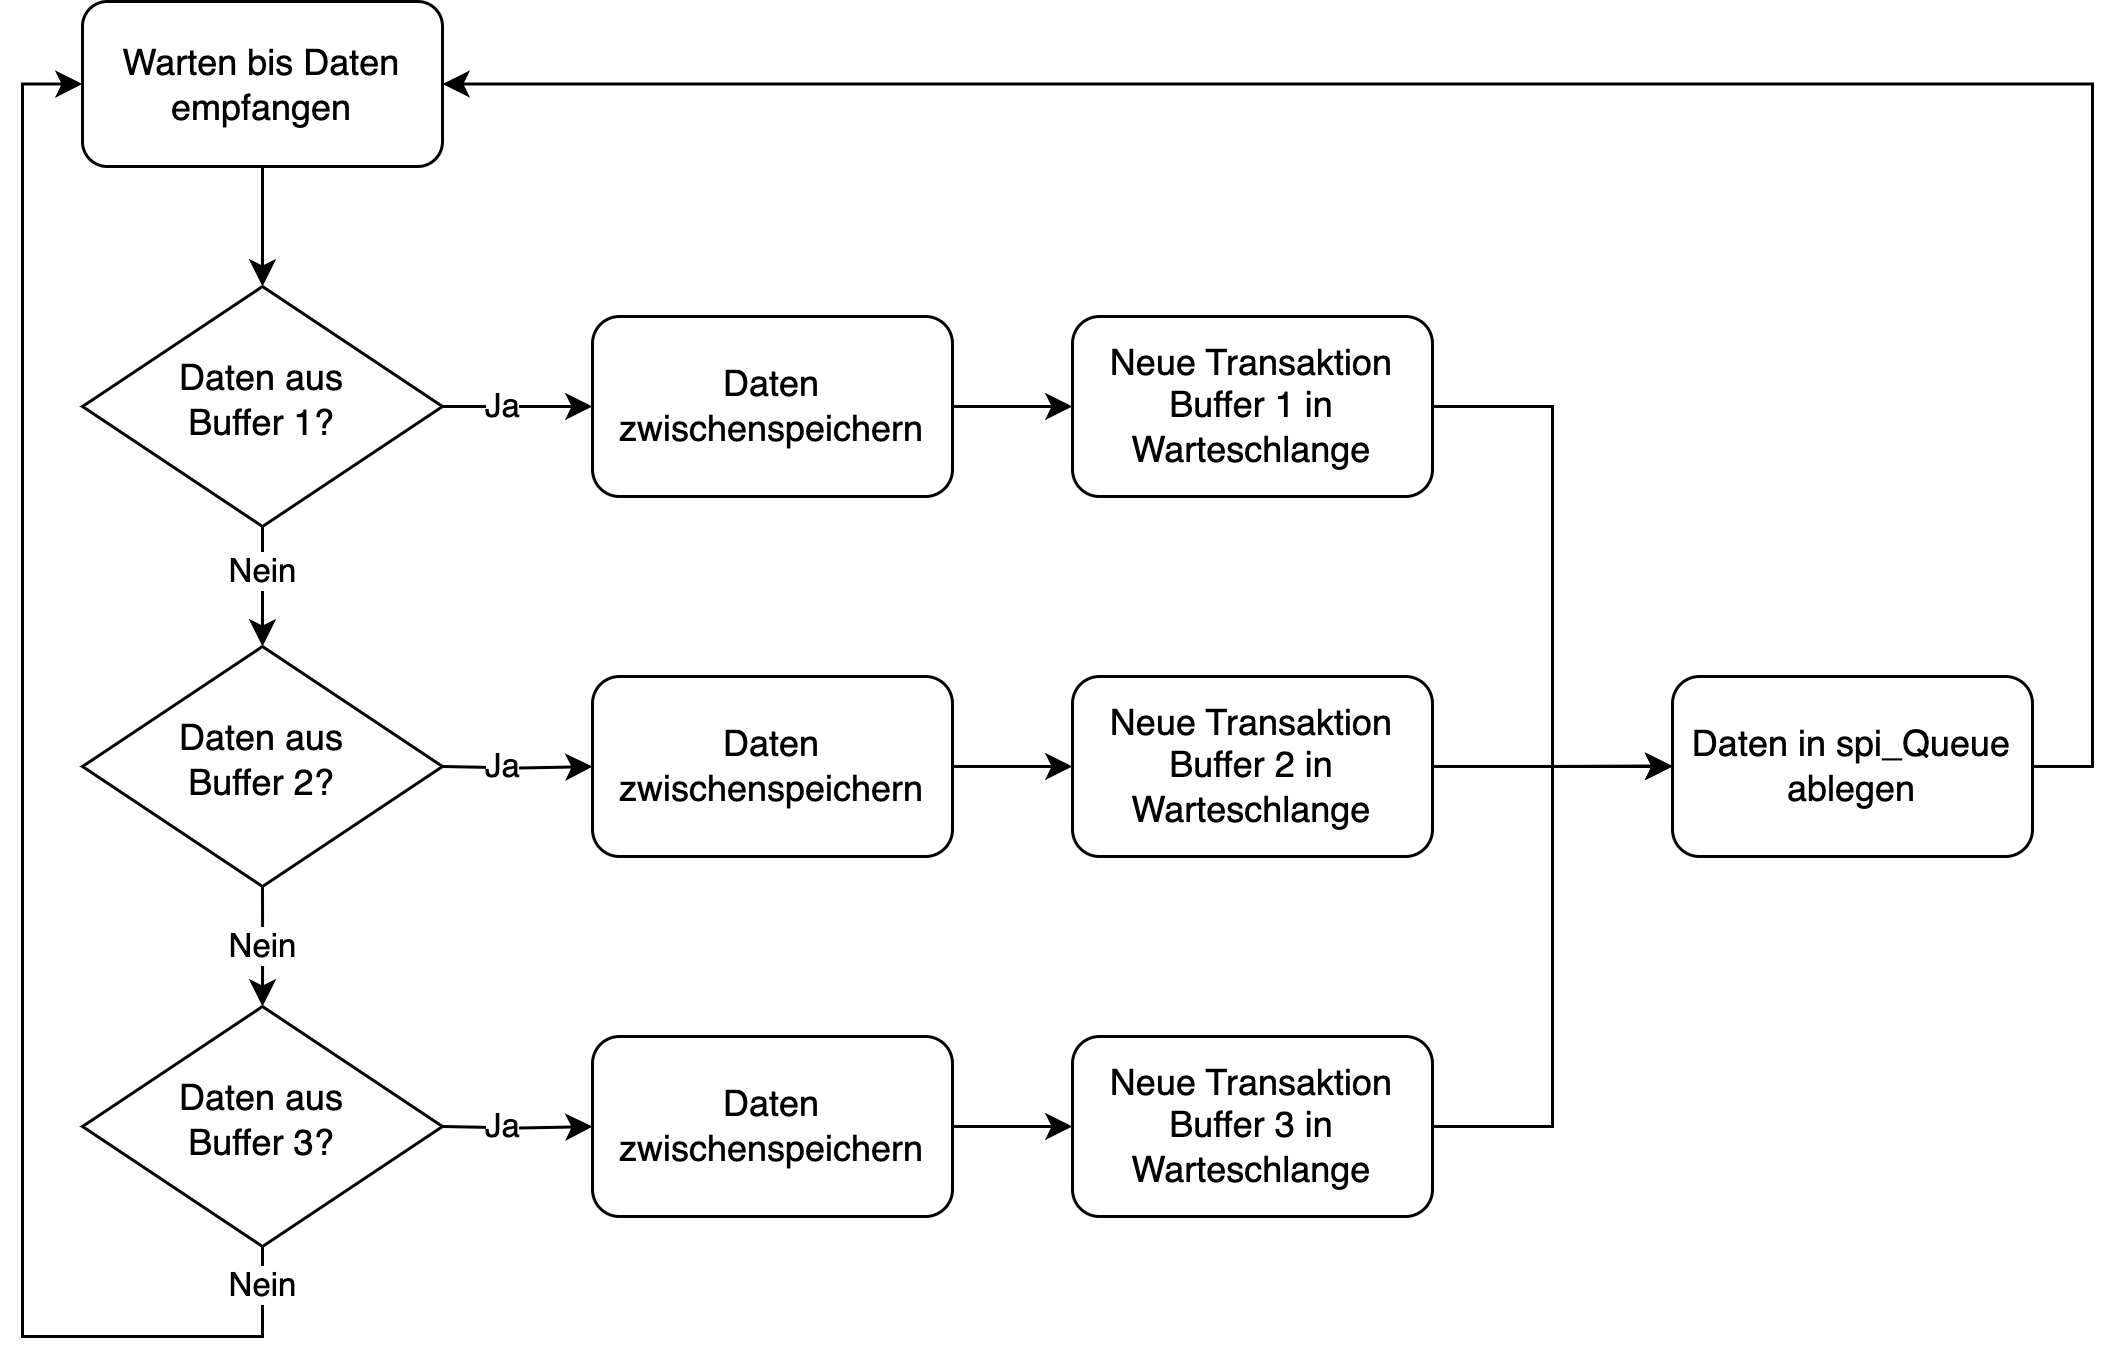
\includegraphics[width=0.75\linewidth]{Figures/Chap3/ESP/SPI_RECEIVE/Bufferkonzept_BLE.png}
    \caption{3-Buffer-Konzept SPI empfangen}
    \label{fig:3BuffKonz}
\end{figure}

Zur Weitergabe der empfangenen Daten in die \textit{spi\_queue} wird die in Kapitel \ref{subsub:UnionSPI} beschriebene Union verwendet.

Der folgende Codeausschnitt zeigt exemplarisch die Verarbeitung eines Buffers, einschliesslich der Nutzung der Union und des Empfangs von Daten:

\begin{lstlisting}[language=C]
/* FreeRTOS TASK */
void spi_receive(void *pvParameters)
{
    //...
    
    while (true)
    {
        // Programm geht nicht weiter, wenn keine Daten Empfangen werden.
        spi_slave_get_trans_result(RCV_HOST, &trx_ptr, portMAX_DELAY);

        // Abgleich Buffer
        if (trx_ptr->user == t1_ptr->user)
        {
            u_message.spi_rec[0] = receive_data1[0];
            u_message.spi_rec[1] = receive_data1[1];
            spi_slave_queue_trans(RCV_HOST, &t1, 0);
        } 
        else if
        {
        // ... Weitere Receive Buffer
        }
        else
        {
            // Daten liegen in keinem Gueltigen Buffer. --> Verwerfen
            // Unterbricht while() schleife hier und startet wieder oben
            continue;
        }
        
        // Beispiel wechsel von Little Endian auf Big Endian
        queue_msg = (u_message.bytes.byte0 << 8 | u_message.bytes.byte1);
        xQueueSend(dataQueue_spi, (void *) &queue_msg, (TickType_t)0);
        // ...
    }
}
        
\end{lstlisting}


\subsection{Task - Decodierung Manchester Signal}
\label{sub:MvbManchDecode}
%\textcolor{red}{Hier wird erklärt, wie die Statemachine für die Decodierung des Manchester Encodierten Signals Verwendet wurde. }
Gemäss Kapitel \ref{sec:HardwareFPGA} werden jeweils acht Nutzdatenbits als 16 Bit Werten transferiert. Dies, um Manchester-Violations zu erkennen, die im Master- und Slave Start-Delimiter vorhanden sind (siehe Kapitel \ref{sub:StartDelimiter}). Die Statemachine verarbeitet pro Durchlauf je acht Nutzdatenbits. Bei einer SPI-Transaktion werden jeweils 32 Nutzdatenbits übertragen. Das bedeutet, dass nach einer Übertragung jeweils vier neue Werte in der spi\_queue vorhanden sind, welche bearbeitet werden. 

Zur Zusammensetzung der Telegramme wurde eine Statemachine implementiert, da die Reihenfolge der Telegramme auf dem Datenbus ideal für dieses Konzept ist. Eine grafische Darstellung der Statemachine findet sich im Ablaufdiagramm im Anhang \ref{app:ManchDec}.

Gemäss Kapitel \ref{sub:MasterSlavePrinzip} wird ein Telegramm in zwei Schritten auf dem Bus gesendet. Als Erstes wird ein Master-Frame mit einer gleichbleibenden Länge von 32 Nutzdatenbits versendet. Die Länge des darauffolgenden Slave-Frames variiert zwischen einer Länge von 32 - 296 Nutzdatenbits.

Damit der Prozess eines Telegramms gestartet werden kann, muss zuerst das Master Start-Delimiter (gemäss Kapitel \ref{sub:StartDelimiter}) erkannt werden. Dies erfolgt anhand der hexadezimalen Repräsentation des Wertes für den Start-Delimiter und lautet 0xC715. Wird ein solcher Wert erkannt, müssen die Daten der nächsten drei Transaktionen den Master-Frame-Daten und der Master-Checksequenz entsprechen.

Nach dem Master-Frame folgt das Slave-Frame, sofern dieses sende-fähig ist und sich angesprochen fühlt. Auf die gleiche Weise wie vorhin wird der empfangende Wert auf seine hexadezimale Repräsentation überprüft. Diese lautet 0xA8E3. Wird diese nicht erkannt, kann dies folgende zwei Gründe haben:

\begin{enumerate}
    \item Anstelle des Slave Start-Delimiters wurde ein Master Start Delimtier geschickt. Dies passiert, wenn der Slave Teilnehmer aktuell nicht bereit zu senden ist. 
    \item Es ist weder ein Master- noch ein Slave Start-Delimiter. Daten sind verloren gegangen, jedoch kann nicht zurückgeführt werden, wie viele.
\end{enumerate}

In beiden Fällen wird das aktuelle Telegramm abgebrochen und mit einem entsprechenden Error Code über die ble\_queue (siehe Kapitel \ref{subsub:Queue}) an den Task bt\_send übermittelt. 

Wird der Slave Start-Delimiter erkannt, werden die Slave-Daten und Checksequenzen empfangen. Abbildung \ref{fig:SlaveFrameFormat} zeigt die übertragbaren Nutzdatenbits pro Frame-Grösse. Beispielsweise werden bei einem Frame mit 128 Nutzdatenbits in 8-Bit-Schritten verarbeitet: Zuerst 64 Nutzdatenbits in 8 Zyklen, gefolgt von einer separaten Checksumme. Anschliessend folgen weitere 64 Nutzdatenbits und eine abschliessende Checksumme. Der untenstehende Code zeigt die Implementierung in C. Die Variable \textit{slave\_data\_loop} in der Zeile 8 und \textit{slave\_check\_loop} in Zeile 29 definieren dabei die Anzahl Zyklen und werden im vorherigen Schritt \textit{Slave Start} gemäss Tabelle \ref{tab:SchlaufenSlaveLoops} gesetzt. 

Ist die Bedingung in Zeile 29 \textit{false} wird der aktuelle Pointer auf das Telegramm über die ble\_queue dem Task bt\_send übergeben. 


\begin{lstlisting}[language=C]
// In diesem Case werden die Slave Daten im struct abgespeichert.
case Slave_data:

    // 
    p_current_tel->data_s[cnt_data_loop + (cnt_check_loop << 3)] = get_byte(receivedData);

    // slave_data_loop ist 2, 4, oder 8 (Anzahl Datenbytes, bevor (!) Checksequenz folgt
    if(cnt_data_loop < slave_data_loop-1) 
    {
        cnt_data_loop++;
    } 
    else //wenn 2, 4, 8 bereits erreicht kommt eine Checksequenz
    {
        cnt_data_loop = 0;
        telg_state = Slave_check;
    }
    
    break;

// In diesem Case werden die Slave Checksequenzen im struct abgespeichert.
case Slave_check:

    // 
    p_current_tel->check_s[cnt_check_loop] = get_byte(receivedData);

    cnt_check_loop++;

    // slave_check_loop entweder 1, 2, oder 4 (Anzahl Checksummen)
    if (cnt_check_loop < slave_check_loop)
    {
        telg_state = Slave_data;
    } 
    else 
    {
        // put pointer to queue
        xQueueSend(dataQueue_ble, &p_current_tel, 0);

        // Message buffer increment 
        buff_incr = (buff_incr + 1) % MAX_MESSAGES;

        // Switch to start 
        telg_state = Master_start;
    }

    break;
\end{lstlisting}

\begin{table}[H]
    \centering
    \begin{tabular}{c|c|c}
        Data-Bit & slave\_data\_loop & slave\_check\_loop\\
        \hline
        \hline
        16 & 2 & 1\\
        \hline
        32 & 4 & 1\\
        \hline
        64 & 8 & 1\\
        \hline
        128 & 8 & 2\\
        \hline
        256 & 8 & 4\\
        \hline
    \end{tabular}
    \caption{Anzahl Schlaufen, welche für die gesamte Aufnahme der Daten erforderlich sind}
    \label{tab:SchlaufenSlaveLoops}
\end{table}


Zusammenfassend beschreibt dieses Kapitel die Implementierung einer Statemachine zur effizienten Verarbeitung von Telegrammen, die auf dem Datenbus nach festgelegten Regeln übertragen werden. Durch die klare Trennung von Master- und Slave-Frames sowie die schrittweise Verarbeitung der Daten und Checksummen wird sichergestellt, dass die Integrität der Telegramme gewahrt bleibt. Fehlerfälle werden erkannt und entsprechend gehandhabt, während die Daten zuverlässig über die \textit{ble\_queue} weitergeleitet werden.


\subsection{Task Bluetooth Senden}
\label{sub:TaskBTSend}

Der Task \textit{Bluetooth Senden} übernimmt die Aufgabe, Daten aus der \textit{ble\_queue} zu verarbeiten und über Bluetooth zu übertragen. Der Ablauf gliedert sich wie folgt:

\begin{enumerate}
    \item \textbf{Entnahme des Pointers aus der Queue:}  
    Der Task nimmt einen Pointer aus der \textit{ble\_queue}, der auf die zu sendenden Daten aus dem Telegramm Array verweist.
    
    \item \textbf{Anlegen eines Buffers:}  
    Die Daten werden mit der ble\_hs\_mbuf\_from\_flat()-Funktion in einen lokalen Buffer geladen, um sie für die Übertragung vorzubereiten.
    
    \item \textbf{Notification:}  
    Die Übertragung erfolgt mit der ble\_gatts\_notify\_custom()- Funktion, die die Daten als Notification an verbundene Geräte sendet.
    
    \item \textbf{Zurücksetzen des Buffer-Bereichts:}  
    Nach Abschluss der Übertragung wird der Buffer auf Null gesetzt, um für die nächste Nutzung vorbereitet zu sein.
\end{enumerate}

Dieser Task nutzt die Mechanismen von FreeRTOS und die Funktionen des BLE-Stacks, um die Datenübertragung durchzuführen. Der Host-Driver muss vorab konfiguriert werden. Der Code dafür wurde aus einem Codebeispiel von der ESP-IDF kopiert und gemäss dem eigenen Nutzen angepasst. \cite{BLUETOOTH_EXAMPLE_GATT}



\subsection{Bluetooth GATT-Server}
\label{sub:BluetoothGATT}
%\textcolor{red}{Wie wurde der Bluetooth Gatt-Server aufgebaut. Erklärung Charakteristiken}
Auf dem ESP32-S3 stehen zwei Bluetooth Low Energy Host Systeme zur Verfügung. Der BluFi-Host sowie der NimBle-Host\cite{BLUETOOTH_API}. Für dieses Projekt wurde der NimBle-Host verwendet, da es gut dokumentiert ist und Beispielcode zur Verfügung steht.

In Abbildung \ref{fig:BLEGATT} ist eine grafische Darstellung des Generic Attribute Profile (GATT) Servers zu sehen.

\begin{figure}[H]
    \centering
    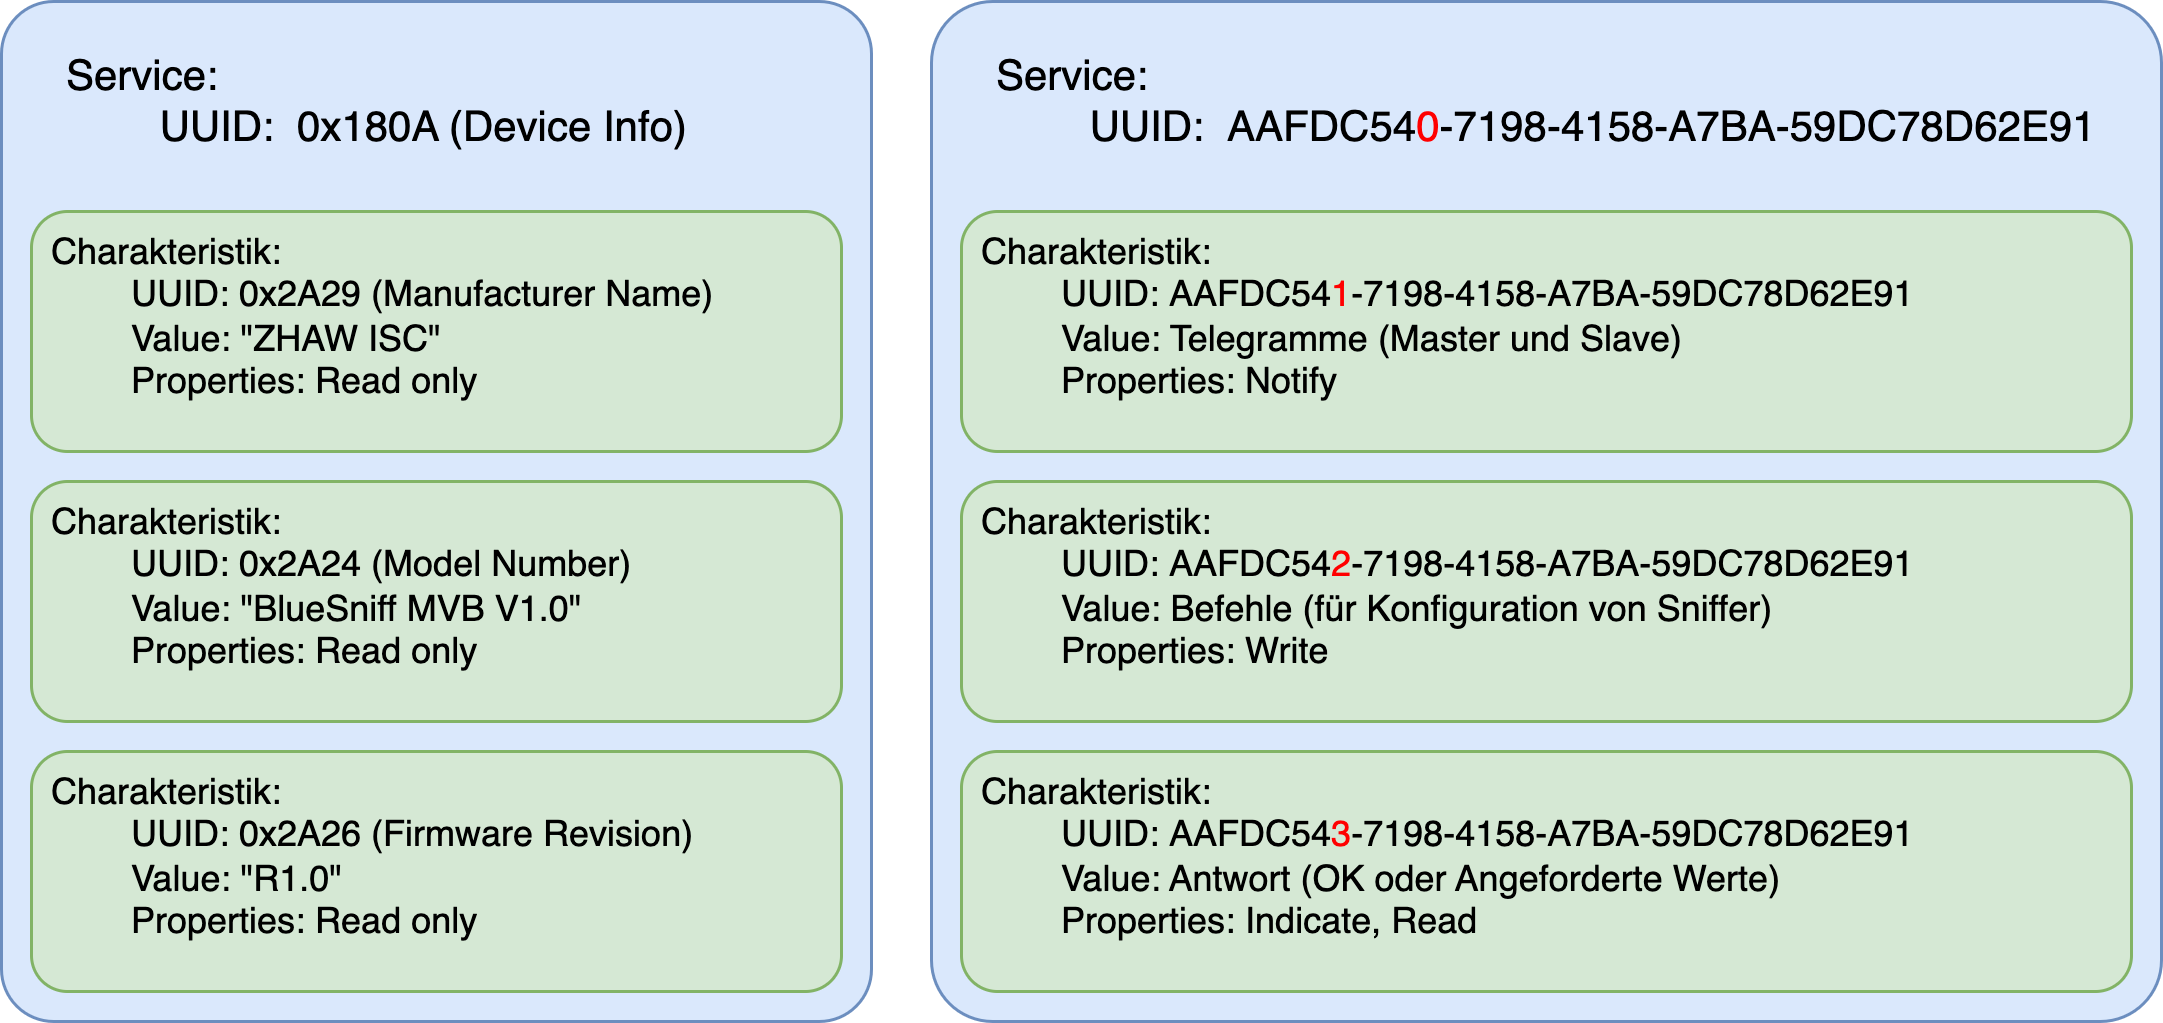
\includegraphics[width=0.9\linewidth]{Figures/Chap3/ESP/BLE/BLE.png}
    \caption{Bluetooth GATT Server auf ESP3-S3}
    \label{fig:BLEGATT}
\end{figure}

\subsubsection{Service - Device Info}
Der Service \textit{0x180A} zur \textit{Device Info} stellt dabei grundlegend statische Werte zur Verfügung, welche die Identifikation des Gerätes mit \textit{0x2A24 Model Number} oder die Aktualität der Firmware \textit{0x2A26 Firmware Revision} nach aussen zur Verfügung stellen. Die aktuellen Werte sind Beispielwerte und werden sich zu einem späteren Zeitpunkt ändern. 

\subsubsection{Service - Sniffer}
Der zweite Service stellt keine vordefinierte 16bit UUID zur Verfügung. Daher wurde diese Service-UUID mithilfe eines \textit{Online UUID Generator} generiert. In Abbildung \ref{fig:BLEGATT} ist die Zahl an 8. Stelle rot markiert. Dies soll darauf hinweisen, dass diese Zahl für die Charakteristiken inkrementiert wurde. Der selbstdefinierte Service soll den Datenaustausch zwischen Sniffer und Endgerät handeln. 

Die Charakteristik mit der roten Zahl 1 soll dabei die empfangenen Telegramme nach aussen schicken. Der erwartete Data-Throughput ist gemäss Kapitel \ref{tab:Busauslastung} bei Übertragung des gesamten MVB-Traffics hoch. Aus diesem Grund ist die \textit{Propertie} dieser Charakteristik auf \textbf{Notify} gesetzt.

Die Charakteristik mit der roten Zahl 2 soll ein individualisierbares Befehlsset schicken können, womit der Sniffer gesteuert, beziehungsweise dessen Verhalten geändert werden kann. Beispiele dazu sind die Einstellung eines Filters oder die Abfrage von Parametern (siehe dazu Kapitel \ref{sec:AusblickFirmwareESP32}). Weil die Befehle auf den Sniffer geschrieben werden, ist die \textit{Propiertie} in diesem Fall \textbf{Write}.

Die Charakteristik mit der roten Zahl 3 soll die Befehle, welche mit der vorherigen Charakteristik geschickt worden sind, mit einer OK-Message bestätigen oder einen Payload haben. Die \textit{Propiertie} ist auf \textbf{Indicate} gesetzt, sodass der Sniffer eine Rückmeldung schickt, sobald er diese bereit hat. Im Falle eines Timeouts kann das Endgerät auch einen \textbf{Read} auf die Charakteristik machen.



\subsection{Datenablage Code}
\label{sub:DatenablageCodeESP32S3}
Das gesamte Projektfile ist im Anhang \ref{app:Ordner41} beigefügt worden. Im Ordner "main" sind 3 Files ersichtlich, die hier kurz erläutert werden.
\begin{itemize}
    \item \textbf{Sniffer\_FW.c}: Das main() File mit dem Einstiegspunkt in der Funktion \textit{app\_main()}.
    \item \textbf{gatt\_svr.c}: Der selbst erstellte GATT-Server gemäss Kapitel \ref{sub:BluetoothGATT}.
    \item \textbf{gatt\_svr.h}: Das Header File zu gatt\_svr.c
\end{itemize}

Das File "'sdkconfig"' entspricht der aktuellen Konfiguration des Projektes. Dort sind beispielsweise die NimBle-Einstellungen ersichtlich und können geändert werden. 